\documentclass[tikz,border=5pt]{standalone}
\pdfinfoomitdate=1
\pdftrailerid{}
\pdfsuppressptexinfo=-1
\usepackage{tikz}
\usetikzlibrary{arrows.meta,positioning}
\definecolor{atlasBlue}{HTML}{0072B2}
\definecolor{atlasGreen}{HTML}{009E73}
% NATO SERS F19; data_sha256=e5716e59343d189b0db914ff58f05ee29a59d8067414da8e1061290811dc8121
% (S) RQ-P01; PP-U-MIN; R_MIN_400_1800; 598 spectra / 69 physical masters.
\begin{document}
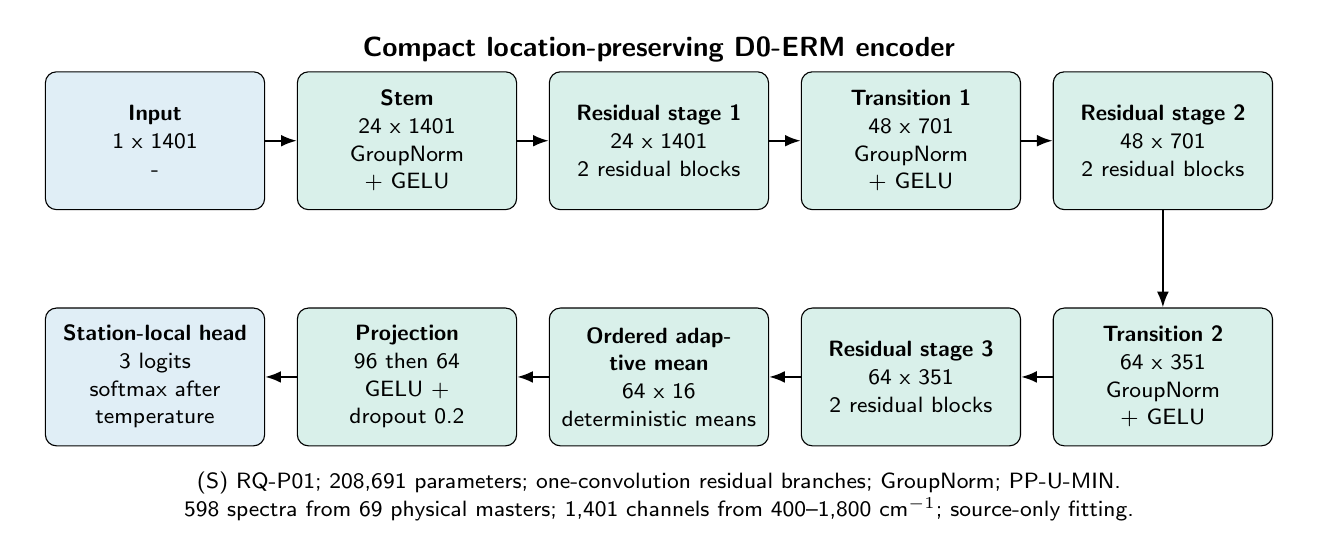
\begin{tikzpicture}[x=1cm,y=1cm,layer/.style={draw,rounded corners,text width=2.55cm,minimum height=1.75cm,align=center,font=\sffamily\fontsize{8}{10}\selectfont},flow/.style={-{Latex[length=2mm]},thick}]
\node[layer,fill=atlasBlue!12] (n0) at (0.0,0) {\textbf{Input}\\1 x 1401\\-};
\node[layer,fill=atlasGreen!15] (n1) at (3.2,0) {\textbf{Stem}\\24 x 1401\\GroupNorm + GELU};
\node[layer,fill=atlasGreen!15] (n2) at (6.4,0) {\textbf{Residual stage 1}\\24 x 1401\\2 residual blocks};
\node[layer,fill=atlasGreen!15] (n3) at (9.600000000000001,0) {\textbf{Transition 1}\\48 x 701\\GroupNorm + GELU};
\node[layer,fill=atlasGreen!15] (n4) at (12.8,0) {\textbf{Residual stage 2}\\48 x 701\\2 residual blocks};
\node[layer,fill=atlasGreen!15] (n5) at (12.8,-3) {\textbf{Transition 2}\\64 x 351\\GroupNorm + GELU};
\node[layer,fill=atlasGreen!15] (n6) at (9.600000000000001,-3) {\textbf{Residual stage 3}\\64 x 351\\2 residual blocks};
\node[layer,fill=atlasGreen!15] (n7) at (6.4,-3) {\textbf{Ordered adaptive mean}\\64 x 16\\deterministic means};
\node[layer,fill=atlasGreen!15] (n8) at (3.2,-3) {\textbf{Projection}\\96 then 64\\GELU + dropout 0.2};
\node[layer,fill=atlasBlue!12] (n9) at (0.0,-3) {\textbf{Station-local head}\\3 logits\\softmax after temperature};
\draw[flow] (n0) -- (n1);
\draw[flow] (n1) -- (n2);
\draw[flow] (n2) -- (n3);
\draw[flow] (n3) -- (n4);
\draw[flow] (n4) -- (n5);
\draw[flow] (n5) -- (n6);
\draw[flow] (n6) -- (n7);
\draw[flow] (n7) -- (n8);
\draw[flow] (n8) -- (n9);
\node[font=\sffamily\bfseries,anchor=south] at (current bounding box.north) {Compact location-preserving D0-ERM encoder};
\node[font=\sffamily\fontsize{8}{10}\selectfont,anchor=north,align=center,text width=15.8cm] at ([yshift=-2mm]current bounding box.south) {(S) RQ-P01; 208,691 parameters; one-convolution residual branches; GroupNorm; PP-U-MIN.\\598 spectra from 69 physical masters; 1,401 channels from 400--1,800 cm$^{-1}$; source-only fitting.};
\end{tikzpicture}
\end{document}
